% This is LLNCS.DEM the demonstration file of
% the LaTeX macro package from Springer-Verlag
% for Lecture Notes in Computer Science,
% version 2.2 for LaTeX2e
%
\documentclass[oribibl]{llncs}
%
\usepackage{makeidx}  % allows for indexgeneration
\usepackage{epsfig}
%

\title{Engineering the Presentation Layer of Adaptable Web Information Systems}
\author{Zolt\'an Fiala\inst{1}, Flavius Frasincar\inst{2}, Michael Hinz\inst{1}, \\ Geert-Jan Houben\inst{2}, Peter Barna\inst{2}, Klaus Meissner\inst{1}}

\institute{Technische Universit\"at Dresden\\ Mommsenstr. 13, D-01062, Dresden, Germany  \\ 
\email{\{zoltan.fiala,mh5,kmeiss\}@inf.tu-dresden.de} \and Technische Universiteit  Eindhoven\\ PO Box 513, NL-5600 MB, Eindhoven, The Netherlands \email{\{flaviusf,houben,pbarna\}@win.tue.nl}}



\begin{document}
\maketitle


\begin{abstract}
Engineering adaptable Web Information Systems (WIS) requires systematic design models and specification frameworks. 
A complete model-driven methodology like Hera distinguishes between the conceptual, navigational, and presentational aspects of WIS design and identifies different adaptation ``hot-spots" in each design step.
This paper concentrates on adaptation in the presentation layer and combines the modeling power of Hera with the versatile presentation capabilities of the AMACONT project.
After discussing different aspects of presentation layer adaptation, the layout manager mechanism of 
AMACONT for describing the adaptable layout of ubiquitous Web presentations is introduced. 
Then the RDFS-based Hera schema for presentation models is presented, allowing to assign AMACONT layout descriptors to Hera slices. 
According to this formalization, Hera application model instances are automatically transformed to a component-based AMACONT implementation that can be adjusted to different end devices and output formats.
The XML-based transformation process is explained in detail, and the resulting methodology is exemplified by a prototype application.
\end{abstract}


\section{Introduction}
Engineering \emph{personalized} Web Information Systems (WIS) is a complex process that has to be based on disciplined, systematic methodologies.
Among these we distinguish the model-based methodologies due to the numerous benefits they offer: easy system analysis, modular decomposition, adaptation ``hot-spots", flexibility, maintainability etc.
By identifying crucial phases of Web development, such an approach helps designers and programmers to proceed in a structured way.

Hera~\cite{hera:jwe} is a model-driven design methodology and specification framework focusing on the development of personalized WIS.
Based on the principle of separation of concerns it distinguishes three design steps: \emph{conceptual design}, \emph{navigational design}, and \emph{presentation design}. 
At each design step different aspects of adaptation can be specified in terms of formal models~\cite{hera:itcc}. 
In order to make the semantics of models explicit, Hera uses RDF(S)~\cite{rdf,rdfs}. 
RDFS inheritance mechanism proved to be useful for reusing 
different design artifacts~\cite{hera:itcc}. 
However, previously Hera's presentation model has not been formalized, nor was adaptation at 
the presentation level implemented in the Hera tools.

%The AMACONT\footnote{AMACONT stands for "System Architecture for Multimedia Adaptive Web CONTent"}
The AMACONT project~\cite{amacont:jwe} recently introduced a \emph{component-based XML document format}. 
It enables to compose personalized ubiquitous Web presentations 
from reusable document components encapsulating adaptive content, behavior, 
and layout. 
A special focus of AMACONT lies on the presentation layer of adaptive Web 
applications. 
It allows to describe the layout of adaptable Web components in a device independent way.
Furthermore, a document generator for adjusting those components to different formats and devices has been developed.

Taking advantage of the analogies between Hera's \emph{slices} and AMACONT's \emph{components}, this paper aims at combining the modeling power of Hera with the presentation capabilities provided by AMACONT.
The AMACONT concept of abstract \emph{layout managers} is adopted for the presentation model of Hera, and its RDFS-based formalization is provided.
According to this formalization of the presentation model, Hera specifications can now be automatically transformed to AMACONT's adaptable Web components.

The paper is structured as follows.
After addressing related work and different aspects of 
presentation level adaptation in Section~\ref{pres_adapt}, a
short overview of the model-driven Hera specification framework is given
in Section~\ref{hera}. 
Section~\ref{amacont} explains the layout manager mechanism of AMACONT in detail.
Finally, Section~\ref{transformation} introduces the formalized Hera presentation model schema and depicts the 
%XML-based process of automatically transforming Hera application model instances to adaptable AMACONT components.
overall data transformation and presentation generation process.
As a proof of concept the proposed methodology was implemented for an art museum WIS. 
To help the reader grasp the different models, graphical excerpts are provided for the different RDFS model representations. 

\section{Presentation Layer Adaptation}
\label{pres_adapt}

\subsection{Presentation Design}
Recently, different approaches for modeling hypermedia or Web applications have emerged.
Among the most significant contributions besides Hera we mention the Object Oriented Hypermedia Design Model (OOHDM~\cite{oohdm}), the Web Modeling Language (WebML~\cite{ceri:webml}), the UML-based Web Engineering approach (UWE~\cite{uwe}), Object-Oriented Web-Solutions Modelling (OOWS~\cite{oows2003}), and the Object-Oriented Hypermedia Method (OO-H~\cite{oo-h2003}).
Even though utilizing different formalisms and notations, all these methodologies are similar in distinguishing among (1) the \emph{conceptual} design of the application domain, (2) the \emph{navigational} design defining the (abstract navigational) structure of the hypermedia presentation, and (3) the \emph{presentation} design specifying the rendering of navigation objects (layout).

\emph{Presentation design} aims at declaring the ``look-and-feel" of a Web application independent from its implementation. 
For this reason, some WIS methodologies use explicit models allowing to compose the layout of Web presentations from abstract user interface elements (also called \emph{abstract data views} in OOHDM or \emph{user interface views} in UWE).
On the other hand, methods like WebML do not include a specific model for expressing presentation at the conceptual level and hide the presentation in application specific XSLT stylesheets.
The drawback of the latter approach is that system maintenance becomes difficult.

As a significant approach for the automatic generation of Web-based multimedia presentations we mention the Cuypers engine~\cite{cuypers2001}. 
Its presentation design uses Prolog rules declaring qualitative and quantitative constraints on the spatial and temporal arrangement of presentation elements.
Though being very flexible, the lack of an explicit model makes it difficult to predict (or enforce) how the presentation should look like in the end of the generation process.
Recently, Cuypers was enhanced by a multimedia formatting vocabulary for explicitly specifying the visual layout of multimedia presentations.
Similar to the well-proven layout management of \TeX, it allows to adjust presentation elements according to a top-to-bottom (\texttt{vbox}) or a left-to-right (\texttt{hbox}) order.
Still, more difficult arrangements (like the layout managers \texttt{GridLayout}, \texttt{BorderLayout}, or \texttt{OverlayLayout} from the Java AWT libraries) are not supported, yet.

In recent years, different XML-compliant user interface descriptions languages, like UIML and XIML have emerged~\cite{souchon2003}.
However, besides abstract layout specification they also aim at modeling other UI aspects, such as domain objects, user tasks, or dialogs.
In Human-Computer Interaction research user interface design has often not
been integrated with the earlier stages in WIS design.
Similar to the Cuypers approach, constraint-based techniques for dynamically adjusting abstract XML presentation descriptions to the displays of mobile devices are discussed in \cite{eisenstein2001}.

\subsection{Adaptation in Presentation Design}
As \emph{personalization} and \emph{adaptation} become prominent issues of WIS design, we claim that it is inevitable to include adaptation aspects in presentation design. 
Still, whereas adaptation has been extensively considered in conceptual and navigational design~\cite{hera:itcc,ceri:webml}, 
adaptation in the presentation layer has not yet been a central issue of WIS methodologies.
Nevertheless, in order to support users' different layout preferences and 
client devices,
different adaptation aspects have to be specified in presentation design.

\begin{itemize}
\item Firstly, it is important to adjust \emph{media instances} to varying technical system parameters provided by different network environments and client devices, such as bandwidth, display resolution, or color depth.
In order to consider such differences, variants of selected media items have to be provided with different quality.
\item A further adaptation target is the corporate design (the ``look-and-feel") of the Web presentation. 
As an example, in an online shop it is common to provide different design variants according to different user properties (age, education, interests, visual impairments etc.) but also according to external parameters (seasons, events, anniversaries etc.).
Depending on these aspects, design elements such as background colors, fonts (size, color, type), or buttons can be varied.
\item Finally, the \emph{spatial} and \emph{temporal} adjustment of layout elements is also an important personalization issue.
Depending on the screen size, the supported document formats, and the interaction techniques provided by different client devices, the presentation components should be displayed accordingly. We mention 3 mechanisms for display adaptation:
(1) \emph{Reorganization}:
In this case the arrangement of media elements on a Web page is adapted.
Whereas for example the tabular arrangement of layout components may look good on conventional desktops, it could cause 
a lot of undesirable horizontal scrolling when being browsed on handhelds with limited display size.
(2) \emph{Exclusion}:
Information being unsuitable for a particular browser (e.g.\ a picture gallery for a monochrome cellphone) or design elements without a semantic meaning (e.g.\ company logos in an online shop) can be excluded from presentations on devices with small displays or low bandwidth connections.
(3) \emph{Separation}:
As an alternative to exclusion, it can be advantageous to put certain content pieces onto separate pages and automatically create hyperlinks to those pages.
This mechanism is very useful to keep the structure of Web pages while providing a lot of information easily understandable on handhelds.
\end{itemize}

The mentioned examples represent static adaptation (also called \emph{adaptability}), i.e.\ an adaptation that does not consider the user's browsing behavior.
However, in some cases it is meaningful to consider dynamic adaptation (\emph{adaptivity}), i.e.\ adaptation according to parameters that may change while the hypermedia presentation is being browsed.
As possible scenarios (in presentation design) we mention the dynamic reorganization of presentation elements on a Web page when the user resizes her browser window or the delivery of alternative media instances when the available bandwidth for a mobile user is decreasing.

\section{The Hera Methodology}
\label{hera}

A typical scenario in a WIS is that in response to a user query the system (semi-) automatically generates a hypermedia presentation.
The generated hypermedia presentation needs to be tailored to the device characteristics and to the user preferences. 
Hera~\cite{hera:jwe} is an example of a model-driven methodology for designing these aspects in a WIS.
%As most of the model-driven
%WIS methodologies Hera distinguishes three models: the conceptual model, which defines the data schema, the application model, which specifies the navigation through the data, and the presentation model, which describes the rendering of the data.
%For the different model representations Hera uses RDF(S)~\cite{rdf,rdfs}, the foundation language of the Semantic Web. 
%RDF flexibility and extensibility fit well with the semistructured nature of Web data. 
%By making the model semantics explicit we better ensure application interoperability.
It proposes a sequence of steps that the WIS designer needs to follow: the conceptual design defining the data schema, the application design specifying the navigation through the data, and the presentation design describing the rendering of the data.
During this entire process, possible adaptation aspects are included
in the associated models \cite{hera:itcc}. 
This section concentrates on two of these models: the conceptual model and the application
model. 
The presentation model (its extended definition) will be described in Section~\ref{transformation}, after
introducing the adaptive layout managers of AMACONT. 

%\subsection{Conceptual Model}
%\label{cm}

The \emph{Conceptual Model} (CM) defines the schema of the data available in the WIS.
It is composed of a hierarchy of concepts and concept relationships.
Concepts have associated attributes that refer to media items.
Figure~\ref{fig:cm} gives an excerpt of the CM for our running example.
Concepts are depicted in dark ovals and contain light ovals which stand for concept attributes. 
In the specification of relationship cardinalities the `Set' construct is used on the side of the concept
that can have more than one instance associated to one instance of the other concept. 
%A standard database technique is used to decompose many-many relationships into %two one-many relationships.

\begin{figure}[h]
\centering
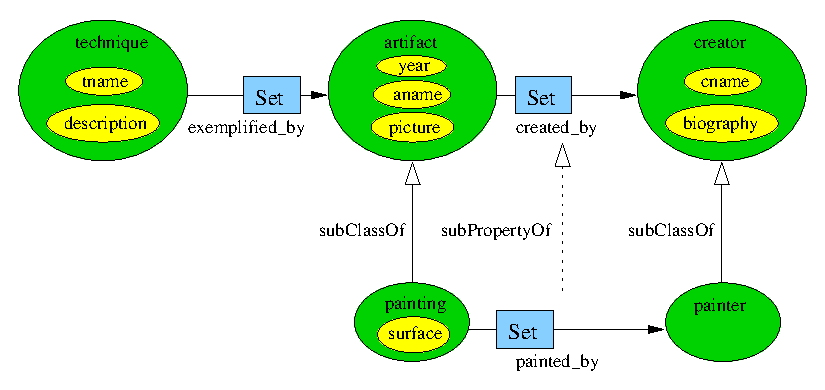
\epsfig{file=cm.eps,width=3.7in}
\caption{The conceptual model}
\label{fig:cm}
\end{figure}

The media types associated to the concept attributes are described in the
\emph{Media Model} (MM), a submodel of CM. MM is a hierarchical model composed of
media types. The most primitive media types are: Text, Image, Audio, and Video.  
Figure~\ref{fig:mm} shows an excerpt of the MM for our running example.
Media types are depicted in dark rectangles.

Adaptation in the CM is based on the \emph{conditional inclusion} of elements. 
Arbitrary complex conditions referencing (ranges of) data describing the 
device capabilities and user preferences can be used. As we do specify 
these conditions as XSLT conditions their expressive power is equivalent 
to the expressive power of XSLT conditions.
This information is stored in a \emph{user profile} containing attribute-value pairs according to a CC/PP~\cite{ccpp} vocabulary. 
The light rectangles in Figure~\ref{fig:mm} depict two adaptation conditions considering screen size constraints. 
One condition
requires that a long text for the technique description and a large image for the
artifact pictures is used for PCs. 
The other condition stipulates that a short text for the technique description and a small image for 
the artifact pictures is used for PDAs.
Remember that the selection of content variants with different quality is an important means of device adaptation.

\begin{figure}[h]
\centering
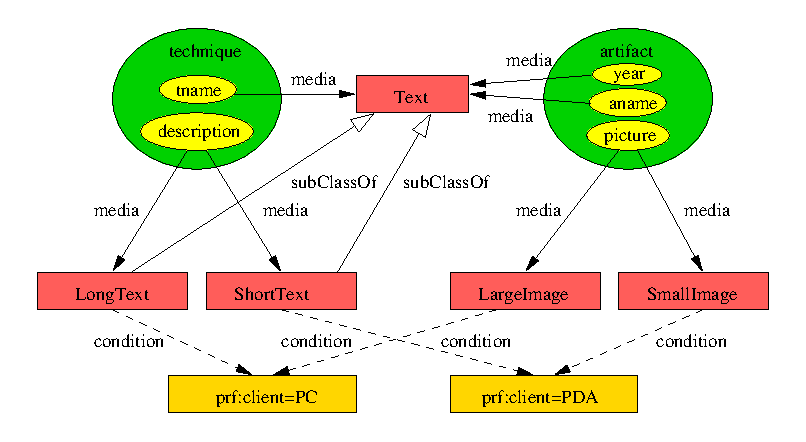
\epsfig{file=mm.eps,width=3.7in}
\caption{The media model}
\label{fig:mm}
\end{figure}

%\subsection{Application Model}
%\label{am}

The \emph{Application Model} (AM) specifies the navigational aspects of the
application. 
It is based on the notion of a \emph{slice} which is a meaningful
grouping of concept attributes that need to be shown together in the
hypermedia presentation. 
A slice can be viewed as a presentation attribute associated to 
a concept. 
In this way the AM is an extension of the CM that provides a view over the CM.

The AM is composed of a hierarchy of slices and \emph{slice relationships}.
There are two kinds of slice relationships: compositional relationships
(aggregation between slices) and navigational relationships (navigation
between slices). 
If a compositional slice relationship relates slices associated with two different concepts, then the CM relationship involved in the composition needs to be specified. 
Figure~\ref{fig:am} shows an excerpt of the AM for our running example.
Slices are depicted (as their name suggests) by pizza-slice shapes.
Hierarchical relationships between slices are omitted here due to lack of
space (we refer the reader to~\cite{hera:itcc} for details on this
matter). 
In complete analogy to the CM, adaptation issues in the AM can be defined by 
attaching \emph{appearance conditions} to slices.

\begin{figure}[h]
\centering
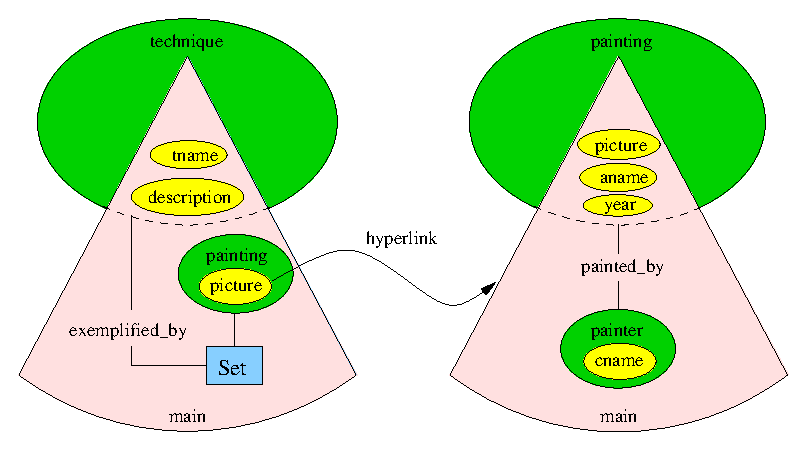
\epsfig{file=am.eps,width=3.7in}
\caption{The application model}
\label{fig:am}
\end{figure}

\section{AMACONT's Component-based Document Model}
\label{amacont}

The component-based document format of AMACONT~\cite{amacont:jwe} aims at building personalized ubiquitous Web applications by aggregating and linking \emph{configurable document components}. 
These components are instances of an XML grammar representing adaptable content on different abstraction levels, i.e.\ layers in AMACONT (see Figure~\ref{docmod}).
\emph{Media components} encapsulate concrete media assets by describing them with technical metadata. 
\emph{Content units} group media components by declaring their layout in a device-independent way. 
Finally, \emph{document components} define a hierarchy out of content units to fulfill a specific semantic role. 
The \emph{hyperlink view} for defining typed links is spanned over all component layers.
%Components' interfaces are described by metadata specifying their properties %and their adaptive behavior. 
For a detailed introduction to the document model the reader is referred to~\cite{amacont:jwe}.

\begin{figure}[h]
\centering
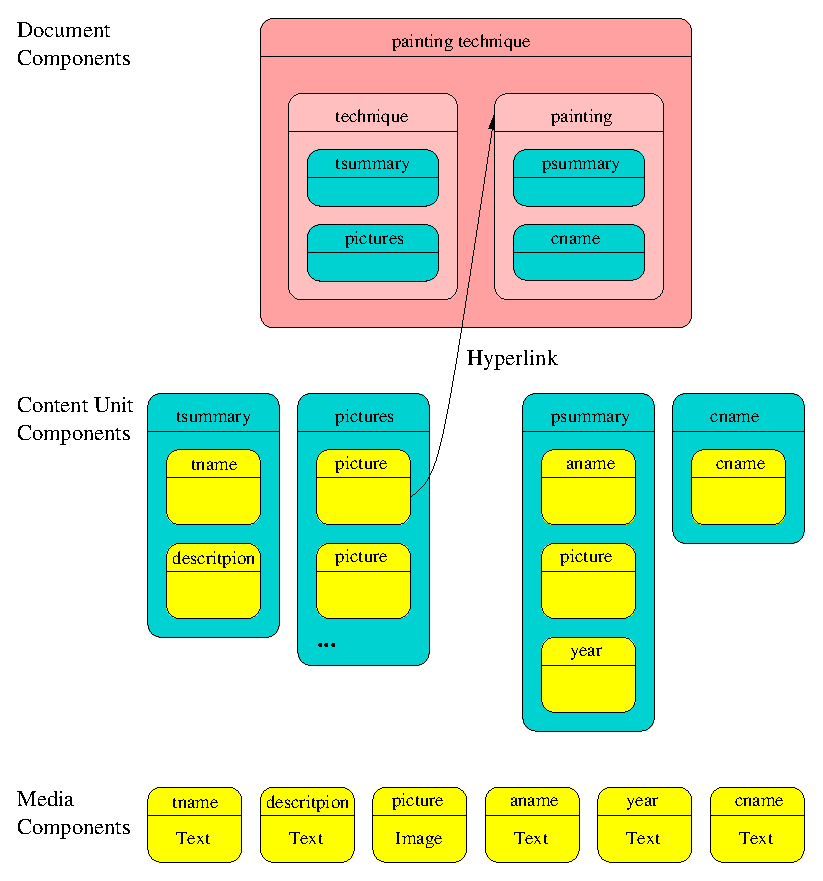
\epsfig{file=dm.eps,width=3.5in}
\caption{The document model}
\label{docmod}
\end{figure}

%\subsection{Describing Adaptive Layout in AMACONT}
%\label{amalayout}

In order to describe the \emph{presentation} of component-based Web documents, 
AMACONT allows to attach XML-based layout descriptions \cite{amacont:jwe} 
to components. 
Inspired by the layout manager mechanism of the Java language (AWT, Swing) 
and the abstract user interface representations of UIML or 
XIML~\cite{souchon2003}, they describe a client-independent layout 
allowing to abstract from the exact resolution of the browser's 
display\footnote{In contrast to UIML or XIML, AMACONT offers a light-weight 
solution that focuses only on the rendering of components and not on other 
aspects like tasks, domain objects, or dialogs, that can be effectively dealt with in the CM or AM.}. 
Furthermore, they also enable to declare simple presentation layer adaptation rules.
Note that layout managers of a given component only describe the presentation of its immediate subcomponents which 
encapsulate their own layout information in a standard component-based way.

Currently four layout managers are defined.
\texttt{BoxLayout} lays out multiple components either vertically or horizontally. 
\texttt{BorderLayout} arranges components to fit in five regions: north, south, east, west, and center. 
It was chosen because it strongly resembles the structure of many Web pages consisting of a header, an optional footer, a main area and one or two sidebars.
\texttt{OverlayLayout} allows to present components on top of each other. 
Finally, \texttt{GridLayout} enables to lay out components in a grid with a configurable number of columns and rows.
Though it can be realized by nested \texttt{BoxLayout}s, we implemented it separately because WISs often present dynamically retrieved sets of data in a tabular way.
The following code snippet depicts the layout description of a content unit containing two media components adjusted by the layout manager \texttt{BoxLayout}. 
An image (aligned right) and a text object (aligned left) are arranged above each other, taking 30 and 70 percent of the available vertical space.

{\small
\begin{verbatim}
<BoxLayout axis="yAxis" border="1">
   <ComponentRef ratio="30%" halign="right">Picture1</ComponentRef>
   <ComponentRef ratio="70%" halign="left">Text1</ComponentRef>
</BoxLayout>
\end{verbatim}
}

Layout managers are formalized as XML tags with specific attributes. 
Two kinds of attributes exist: \textit{layout attributes} and \textit{subcomponent attributes}. 
Layout attributes declare properties concerning the overall layout and are defined in the corresponding layout tags. As an example the \texttt{axis} attribute of \texttt{BoxLayout} determines whether it is laid out horizontally or vertically. 
Subcomponent attributes describe how each referenced subcomponent has to be arranged in its surrounding layout. 
For instance, the \texttt{halign} attribute of \texttt{Picture1} declares it to be right-justified.
Table~\ref{tab:BoxLayoutAttributes} summarizes the possible attributes of \texttt{BoxLayout} by describing their names, role, usage (required or optional) and possible values.

\begin{table}[h]
	\begin{center}
		\begin{tabular}{l l l l}
			\textbf{Layout} &  &  & \\
			\textbf{Attributes} & Meaning & Usage & Values\\
			\hline
			\texttt{axis} & Orientation of the BoxLayout & req. & xAxis$|$yAxis \\	
			\texttt{space} & Space between subcomponents & opt. & int\\	
			\texttt{width} & Width of the whole layout & opt. & string \\	
			\texttt{height} & Height of the whole layout & opt. & string \\													
			\texttt{border} & Width of border between subcomponents & opt. & int \\
			\hline			
			\textbf{Subcomponent} & &  &  \\
			\textbf{Attributes} & Meaning & Usage & Values\\
			\hline
			\texttt{halign} &  Horizontal alignment of subcomponents &  opt.&  left$|$center$|$right\\	
			\texttt{valign} & Vertical alignment of subcomponents &  opt.&  top$|$center$|$bottom\\	
			\texttt{ratio} & Space taken by subcomponent &  opt.&  percentage\\	
			\texttt{wml\_visible} & Should be shown on same WML card? &  opt.&  boolean\\													
			\texttt{wml\_desc} & Link description for WML &  opt.&  string\\	
			\hline						
		\end{tabular}
	\end{center}
	\caption{BoxLayout attributes}
	\label{tab:BoxLayoutAttributes}
\end{table}

Even though most attributes are device independent, we also allowed two platform-dependent attributes in order to consider the specific card-based structure of WML presentations. 
The optional attribute \texttt{wml\_visible} determines whether in a WML presentation the given subcomponent should be shown on the same card.
If not, it is put onto a separate card that is accessible by an automatically generated hyperlink, the text of which is defined in \texttt{wml\_description}.
Note that this kind of content separation (see Section~\ref{pres_adapt}) provides scalability by fragmenting the presentation according to the very small displays of WAP-capable mobile phones. 

The rendering of media objects is done at run time by XSLT stylesheets transforming components with abstract layout properties to specific output formats, such as XHTML, cHTML, and WML. 


\section{Putting it All Together}
\label{transformation}

There are several analogies between \emph{instances} of a Hera application model and \emph{components} in AMACONT.
Both represent meaningful presentation units bearing also some semantic role (e.g.\ painting or painting
technique) and are recursive structures enabling an arbitrary depth of
hierarchy. 
Moreover, both top-level slices and top-level document components correspond to pages to be presented on the user's display and may contain adaptation issues according to device profiles and user profile parameters.
However, in contrast to application model instances AMACONT components also contain adaptive layout information.
Note that layout in Hera is specified in the presentation model (hence, the extensions we made to the definition of this Hera model).

Taking advantage of these analogies and the fact that both Hera and AMACONT rest upon XML, our aim was to combine the modeling power of Hera and the versatile presentation capabilities of AMACONT.
Therefore, the concept of adaptive layout managers was transferred to the Hera \emph{Presentation Model} (PM).
As in AMACONT, they can be assigned to Hera slices in order to declare the arrangement of their subslices in an implementation-independent way.
Furthermore, the PM schema allowing to declare such assignments was formalized in RDFS.
This formalization enables the \emph{automatic mapping} of high-level Hera AM and PM specifications to AMACONT's implementation units, i.e.\ components.

\subsection{PM Schema}

The RDFS-based Hera presentation model supports two mechanisms: the definition of layout managers and their assignment to AM slices.
Based on our running example, the following code snippet from a Presentation Model demonstrates how a layout manager can be assigned to a slice.
The graphical form of this PM is shown in Figure~\ref{pm}.

\begin{figure}[h]
\centering
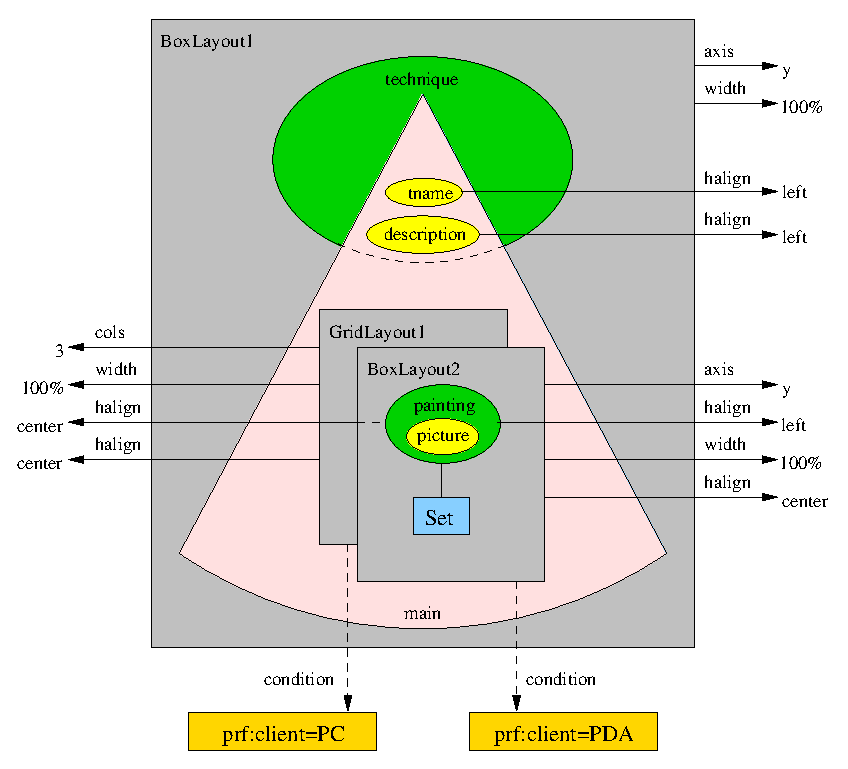
\epsfig{file=pm.eps,width=3.7in}
\caption{A PM example}
\label{pm}
\end{figure}

{\small
\begin{verbatim}
<Slice rdf:about="#Slice.technique.main">
     <layout rdf:resource="#BoxLayout1"/>
</Slice>
\end{verbatim}
}

This assignment rule implies to visualize the slice \texttt{Slice.technique.main} according to the layout manager \texttt{BoxLayout1}.
The following example shows how \texttt{BoxLayout1} is specified in detail.

{\small
\begin{verbatim}
<BoxLayout rdf:id="BoxLayout1">
   <axis>y</axis>
   <width>100%</width>
   <slice-ref rdf:resource="Slice.technique.tname" 
              pres:halign="left"/>
   <slice-ref rdf:resource="Slice.technique.description" 
              pres:halign="left"/>
   <access-element-ref rdf:resource="SetOfLinks_1" 
              pres:halign="center"/>
</BoxLayout>
\end{verbatim}
}

Attributes for components of AMACONT's layout manager (Section~\ref{amacont}) have been adopted to describe the spatial adjustment of subslices.
Both attributes describing the overall layout and attributes specifying the arrangement of each referenced subslice (\texttt{slice-ref}) or access element (\texttt{access-element-ref}) can be defined.
Still, the layout manager of a slice only specifies how its immediate subslices are to be rendered.
%Whenever a subslice has subslices, also, a new layout manager has to be assigned. 
For the access element \texttt{SetOfLinks\_1} the layout specification might 
look like this:

{\small
\begin{verbatim}
<Access-element rdf:about="#SetOfLinks_1">
 <layout rdf:resource="#GridLayout1" 
         pres:condition="pres:client='PC'"/>
 <layout rdf:resource="#BoxLayout2"  
         pres:condition="pres:client='PDA'"/>
</Access-element>\end{verbatim}
}

Note the attribute \texttt{pres:condition} that allows to declare simple \emph{adaptation conditions} that reference parameters from the user/device profile.
Whereas for example the paintings exemplifying the presented painting technique are arranged on a PC in a tabular way (GridLayout1), the small screen size of PDAs requires adjusting them below each other (BoxLayout2).

In contrast to AMACONT's layout managers (defined at instance level), Hera layout assignments have to be specified at \emph{schema level}. 
Due to the dynamic nature of WIS applications, this means that the number of items in an access element is not known at design time.
In such cases one should use either a \texttt{BoxLayout} with an undefined number of cells or a \texttt{GridLayout} so that only one of its dimensions (\texttt{columns} or \texttt{rows}) is predeclared.
The missing dimensions are automatically computed at run time.
 

 


\subsection{The Data Transformation Process}

Figure~\ref{trans2} gives an overview of the data transformation process.
It is composed of four transformation steps that are
described in detail in the rest of this section.

\begin{figure}
\centering
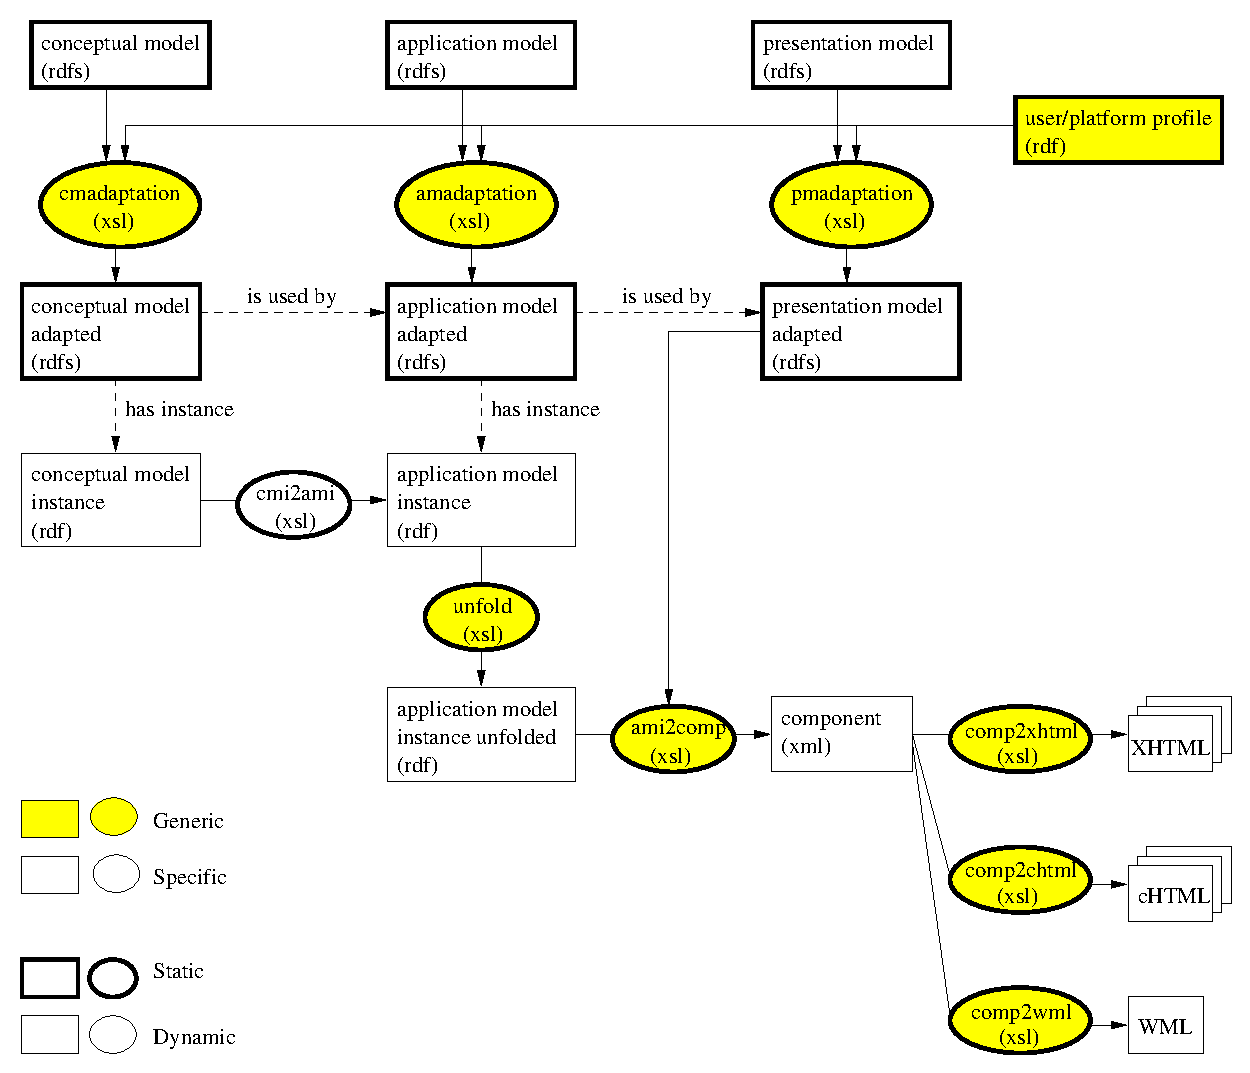
\epsfig{file=transformations.eps,width=4in}
\caption{The data transformation process}
\label{trans2}
\end{figure}

In the first step, based on the attribute values from the user/platform profile, 
the conditions
included in the different models are evaluated. Elements having a
condition evaluated to false are removed from their corresponding models. 
As a result, an adapted conceptual model, an adapted application model, and an 
adapted presentation model are obtained. Note that this adaptation is done at the 
schema level.
The rest of the transformation steps will be performed at the 
instance level (or data level).

The input data to the transformation pipeline is the conceptual model instance.
The gathering of this data in response to a user query is outside the scope
of this paper, see ~\cite{hera:jwe}. In the second step the conceptual model instance is used to 
populate the 
application model. The resulting application model instance represents
the presentation navigational structure.

The third step aims at \emph{mapping} AM instances to adaptable AMACONT components, and is
realized by two transformations substeps.
In the first substep slice composition references are resolved (\emph{unfolding}) and AM instances with hierarchical slice structures (slices containing subslices) are created.
In the second substep the unfolded AM instances are automatically \emph{transformed} to hierarchical AMACONT component structures.
First, top-level slices are mapped to top-level document components.
Then, subslices and their attributes are recursively mapped to subcomponents according to the following rules:

\begin{enumerate}
\item Concept attributes are mapped to media components. 
\texttt{Integer} and \texttt{String} attributes are assigned to text components, media attributes to corresponding media components (image, audio, video etc.).
\item Slices containing concept attributes from a single concept are mapped to single document components containing a content unit that aggregates the corresponding media components.
\item Slices referring to concept attributes and subslices from different concepts are mapped to composite document components containing child document components for each aggregated subslice.
For those subslices this mapping process has to be performed recursively.
\end{enumerate}

The \emph{layout attributes} of the created AMACONT components are \emph{configured} according to the PM schema.
Beginning at top-level document components and visiting their subcomponents recursively, 
the appropriate AMACONT layout descriptors are added to the meta-information section of each component's header.
Since the layout manager attributes of the Hera PM rest upon the layout concepts of AMACONT, this mapping is a straightforward process.
Yet, for access elements (containing a variable number of subslices depending on a dynamic query) the concrete dimensions of \texttt{BoxLayout} or \texttt{GridLayout} 
have to be recalculated for each particular user request.

%The presentation engine aims at publishing the automatically generated AMACONT components to different Web output formats (XHTML, cHTML and WML).
%It was realized by AMACONT's pipeline-based document generator \cite{amacont:jwe}.
%The input components are subdued to two transformation steps.
%The first one interprets AMACONT's abstract layout managers and transforms them to the corresponding output format.
%For instance, a \texttt{BoxLayout} in XHTML is realized by means of a table (and its specific attributes) with either one column or one row.
%However, not all layout managers can be visualized properly on all devices.
%As an example, since palmtops or a WAP phones have very small displays, a horizontal \texttt{BoxLayout} is automatically converted to a vertical arrangement of subcomponents on those devices.
%Similarly, in the case of \texttt{OverlayLayout} only the upper component is presented on handhelds.
%The second transformer resolves references defined in AMACONT's hyperlink view and converts them to hyperlinks of the corresponding format.
%Figure~\ref{output} shows two possible outputs of our running example, one for a PC (XHTML) and another for a PDA (cHTML).

In the last (fourth) step the components are transformed to the corresponding output format.
For instance, a \texttt{BoxLayout} in XHTML is realized by means of a table (and its specific attributes) with either one column or one row.
However, not all layout managers can be visualized properly on all devices.
As an example, since PDAs or WAP phones have very small displays, a horizontal \texttt{BoxLayout} is automatically converted to a vertical arrangement of subcomponents on those devices.
Similarly, in the case of \texttt{OverlayLayout} only the upper component is presented on handhelds.
Figure~\ref{output} shows two possible outputs of our running example, one for a PC (XHTML) and another for a PDA (cHTML).

\begin{figure}
\centering
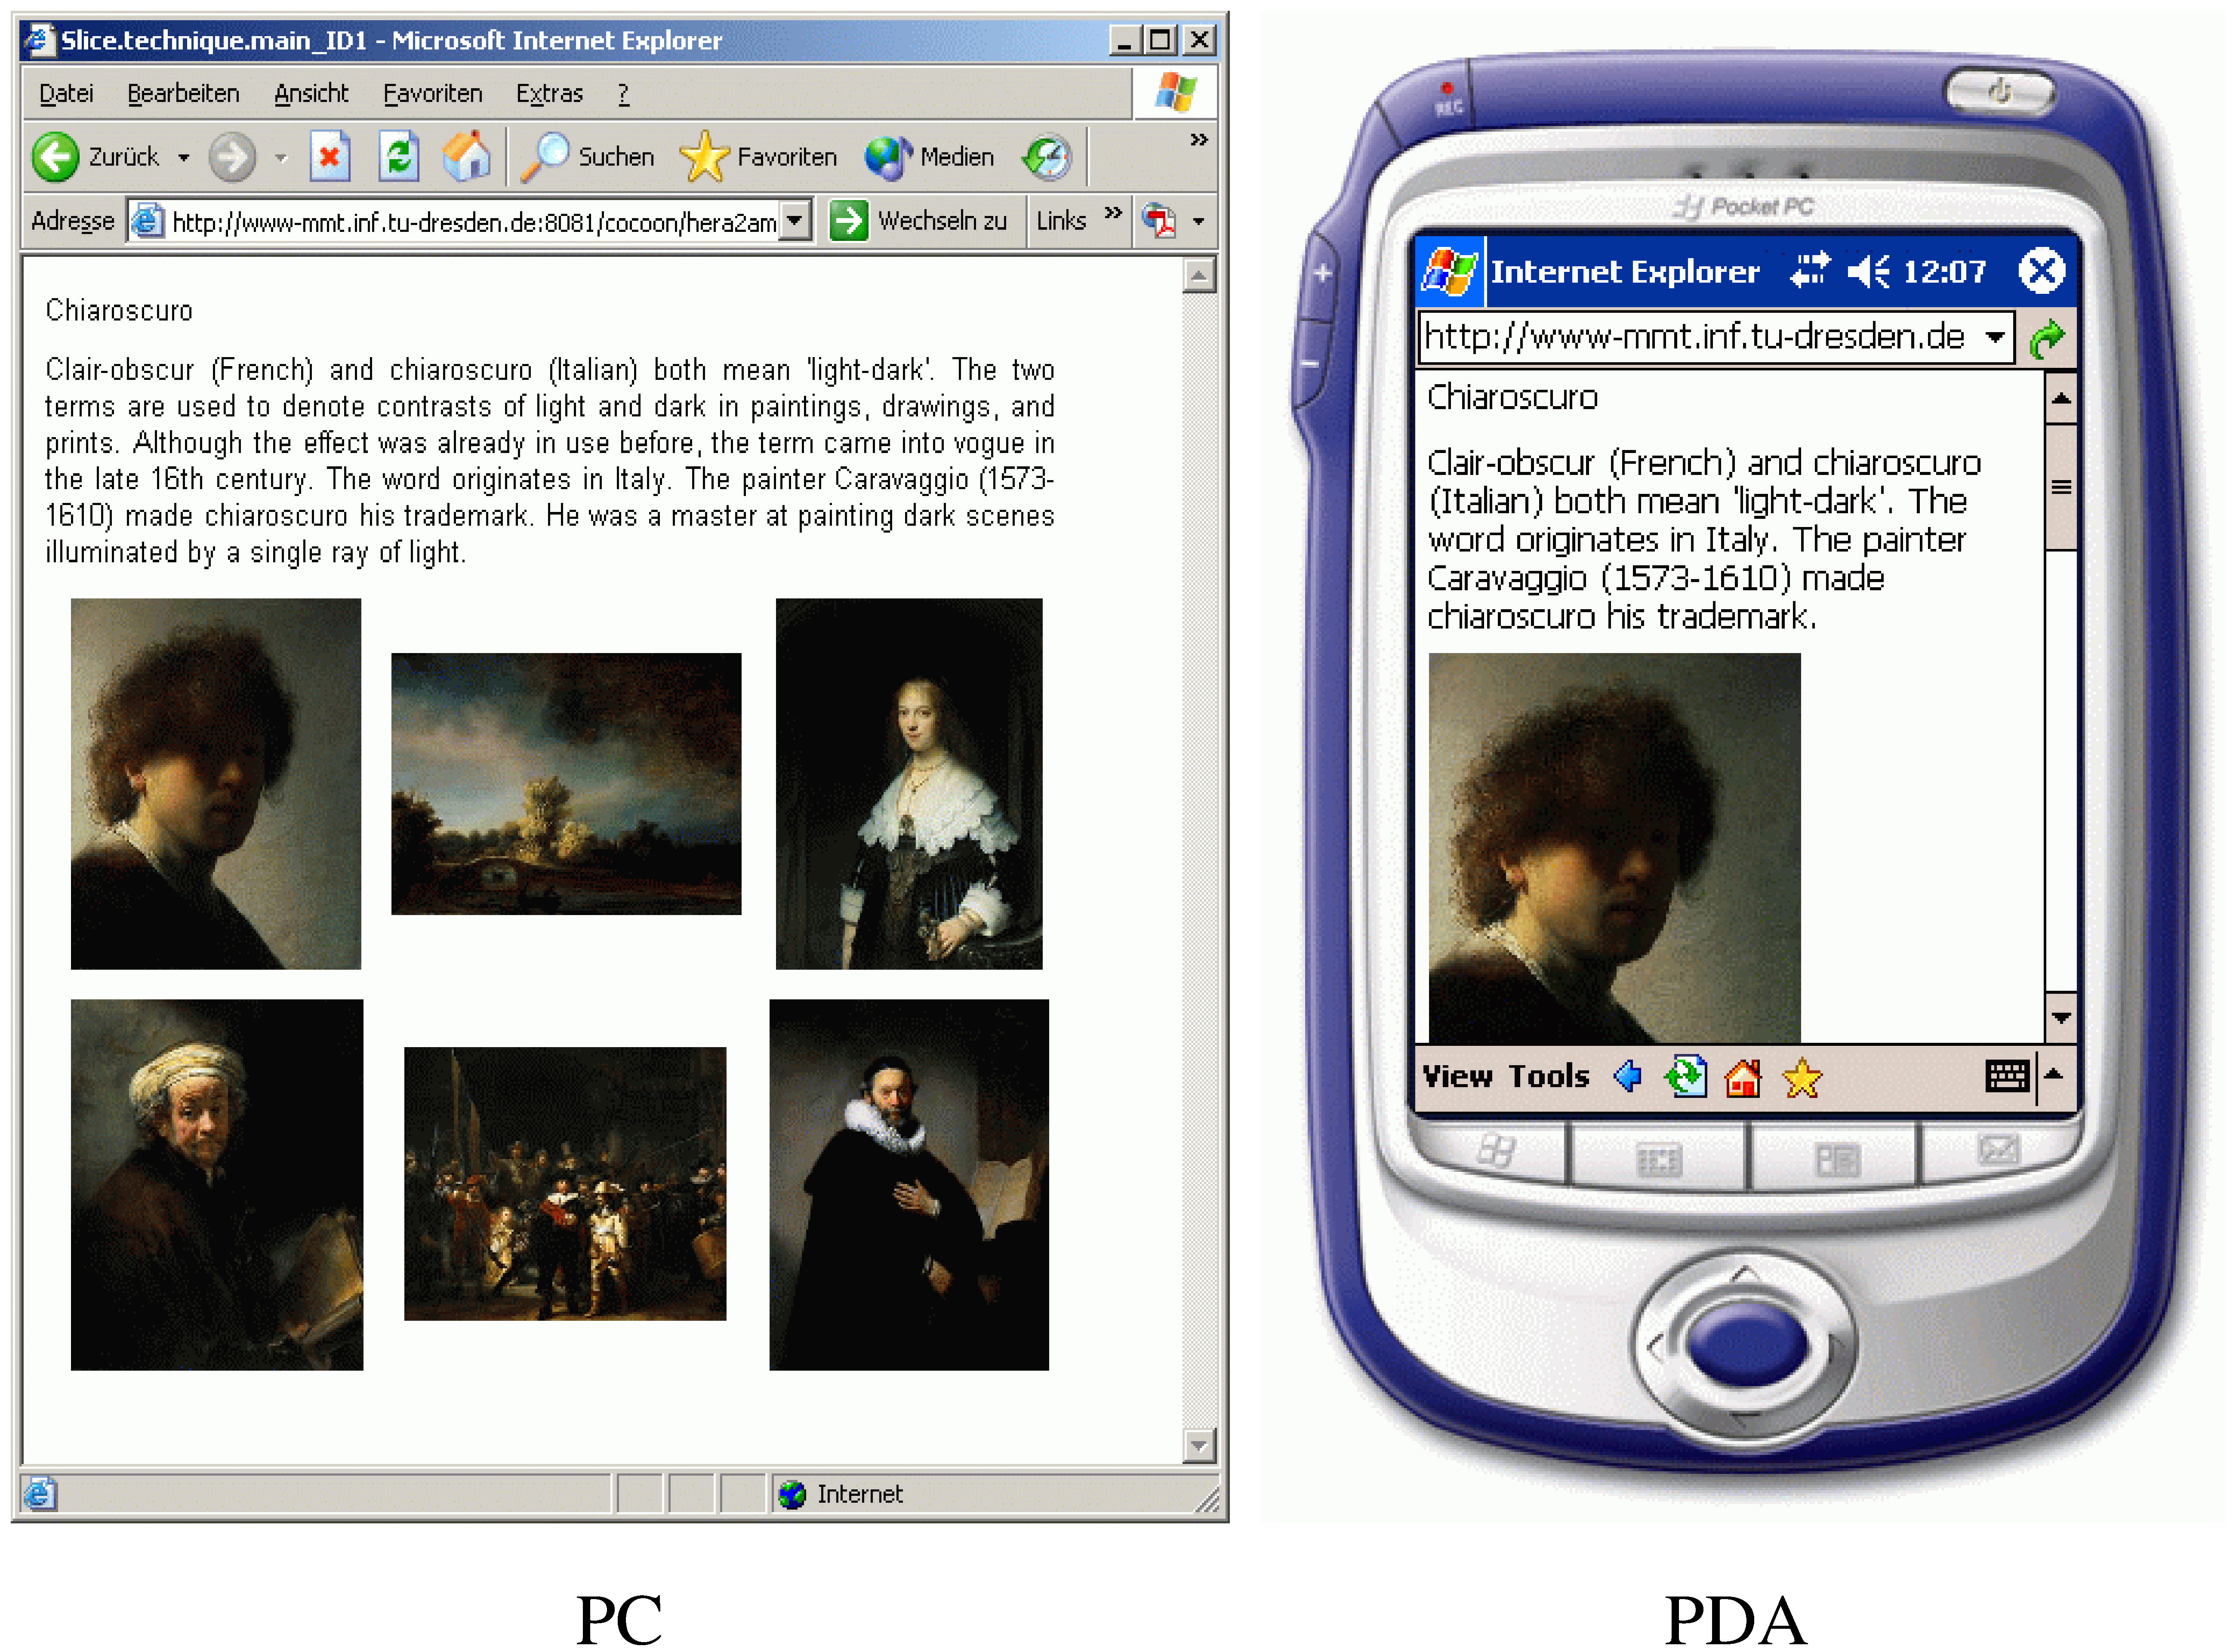
\epsfig{file=presentations.eps,width=4.5in}
\caption{Desktop/PDA presentation}
\label{output}
\end{figure}

\section{Conclusion and Future Work}

In this work we have illustrated the role of presentation layer adaptation in WIS design. 
We have demonstrated how the Hera specification framework (and its implementation tools) can be complemented with the flexible implementation layer provided by the AMACONT project.
Thus these high-level specifications can be mapped to components to be published in different output formats.
It has resulted in an integrated framework (and tool set) that combines the capabilities of Hera at the conceptual and navigation levels with those of AMACONT at the presentation level.

A major focus in ongoing work concentrates on the dynamic coupling of Hera 
and AMACONT.
The static presentation involved in adaptable Web presentations has to be 
enhanced by feedback mechanisms that allow to dynamically react to user's 
browsing behavior.
For this, interactions have to be captured in the generated presentation and sent to the application layer, so that new application model instances can be created and passed back to the presentation layer (engine).
With this extension we will also be able to deal with dynamic adaptation (adaptivity) in the joint system.
%As further matters of future work we mention:


\bibliographystyle{splncs}
\bibliography{r}  

\end{document}

